\documentclass[12pt,a4paper]{article}
\usepackage[utf8]{inputenc}
\usepackage[ngerman]{babel}
\usepackage{graphicx}
\usepackage{amsmath}
\usepackage{hyperref}
\usepackage{color}
\usepackage{cite}

\usepackage[nomarkers,figuresonly]{endfloat}
\makeatletter
\renewcommand\efloat@iwrite[1]{%
   \immediate\expandafter\protected@write\csname efloat@post#1\endcsname{}}
\makeatother
\renewcommand{\efloatseparator}{\mbox{}} 


\newcommand{\HRule}[1]{\rule{\linewidth}{#1}}

\title{ \normalsize \textsc{Semesterprojekt - Dialoge mit Computern}
		\\ [2.0cm]
		\HRule{0.5pt} \\ [0.2cm]
		{\Large \textbf{\uppercase{Athena Bibliotheks-chatbot}}} \\
	    {\large \textbf{\uppercase{Projektbericht}}}
		\HRule{2pt} \\ [0.5cm]
		\normalsize \today \vspace*{5\baselineskip}}

\date{}

\author{
		Matr.: 539911 \\ 
		Dominique Hansen \\
		\and
		Matr.: \\
		Henning Sude \\}



\begin{document}

\pagenumbering{gobble} % Remove and reset page numbering
\maketitle

\clearpage

\tableofcontents
\clearpage

\pagenumbering{arabic} % Reactivate pagenumbering with arabic numbers.

%-------------------------------------------------------------------
% Inhalt ab hier einfügen 
%-------------------------------------------------------------------
\section{Einleitung}

\section{Anforderungsanalyse}

\section{Dialogkonzepte}


\section{Technisches Konzept}


\subsection{Implementierungskonzept}

Das System besteht aus vier Komponenten, die Teilweise wiederum aus Subkomponenten bestehen.%
Alle Komponenten sind mithife von docker kontainerisiert.
Das Setup der Kontainer geschieht mithilfe von docker-compose.
Die Komponenten sind eine PstgreSQL-Datenbank, für die Titeldaten, das User-Interface, dass im backend auch goal handling und den response generator enthält, ein Rasa-NLU server und ein django server, der die Python Module für das Information retrieval, über eine web API, zur Verfügung stellt.
Die Komponenten und ihre Interaktionen sind in Abbildung \ref{fig:architecture_diagram} dargestellt.


\subsubsection{Chatito und Rasa-NLU Trainingsdaten}

\subsubsection{Datenbank}

Zur Speicherung und Bereitstellung der Titel- und Autordaten wurde ein PostgreSQL-Docker-Container mit persistenten volumes für den Inhalt der Datenbank eingerichtet.
Titeldaten wurden von einem frei verfügbaren Datensatz%
\footnote{\url{http://data.ub.tu-dortmund.de/download.html}}
der TU Dortmund genommen und in die Datenbank eingespeist.

\subsubsection{Information Retrieval und Themen Spezifizierung}

Um die Suchfunktion und die spezifizierung eines gesuchten Themas des Chatbots zu implementieren wurden zwei Python Module entwickelt.
Ein Modul stellt Funktionalität zur Suche bereit%
\footnote{Siehe InformationRetrieval in Abb. \ref{fig:class_diagram}}
und das andere ermöglicht es die Themenhierarchie%
 \footnote{Siehe ThematicCategoryDrilldown in Abb. \ref{fig:class_diagram}}
zu durchschreiten.

Die Funktionen zur suche sind so angelegt, dass sie, wenn kein direkter Treffer gefunden wurde, eine liste von fuzzy matches zurückgeben.
Dadurch kann auch bei Tippfehlern oder unvollständigen Suchanfragen ein Ergebnis geliefert werden.
Das Modul zu Themenspezifizierung greift nicht direkt auf die Datenbank zu.
Die Themenhierarchy wird bei der Initialisierung des Moduls in zwei Python Dictionaries geladen.
Eines der Dioctionaries enthält die Klassifikationsummern als keys und die Themennamen als dazugehörige werte.
Die Schlüssel dieses Dictionaries werden benutzt um die hierarchische Beziehung zwischen Themen zu representieren.
Das zweite Dictionairie wird nach dem ersten angelegt und ist eine invertierte Version des ersten.
Hier sind die Themennamen die Schlüsselwerte.
Dieses Dictionarie wird genutzt um die suche nach einem Themennamen zu ermöglichen.


\subsubsection{Frontend}

Das Frontend ist eine HTML/JavaScript-Applikation die von einem nginx Server ausgeliefert wird.
Das Interface, gestaltet mit HTML und CSS und aktualisiert mit jQuery, besteht aus zwei Hälften.
Dem Chat-Fenster in der linken Hälfte und dem Ausgabebereich auf der rechten Hälfte.
Beide befinden sich in CSS-Flexboxen und nehmen unabhängig von der Größe des Fensters die Hälfte des Platzes ein.

Das Chat-Fenster dient als Gesprächs-Log.
Vom Nutzer eingegebener Text wird nach Eingabe dort dargestellt.
Antworten und Begrüßung des Chatbots werden dort ebenfalls dargestellt.
Beide Textarten werden in abgerundeten farbigen rechtecken dargestellt und durch hintergrundfarbe und Bündigkeit unterschieden.
Die Hintergrundfarbe des Chatbots ist Blau, da blau mit einer beruhigenden wirkung in verbindung steht. \cite{Singh2006}
Die beruhigende Wirkung von Blau führt möglicherweise zu einer höheren Bereitwilligkeit nach Misserfolgen weiter zu suchen und könnte dadurch für eine geringere Anzahl von, aus Frustration, abgebrochenen Suchen sorgen.
Antworten des Chatbots sind außerdem linksbündig während die eingaben des Nutzers rechtsbündig sind.
Dies ist dem Aufbau von existierenden Chat-Apps(WhatsApp, Signal, etc.) nachempfunden, in denen eingaben vom Nutzer ebenfalls Rechtsbündig und eingehende Nachrichten linksbündig sind.

Tätigt der Nutzer nach laden des Fensters für 20 Sekunden keine Eingabe, begrüßt Athena den Nutzer von sich aus und erklärt die Möglichkeiten, die dem Nutzer zur Verfügung stehen.
Die Verzögerung dient dazu einem Nutzer, der bereits weiß wie er vorgehen muss, nicht mit unnötigen Erklärungen zu stören.

Eingaben des Nutzers werden zuerst an die Rasa-NLU Schnittstelle gesendet.
Die Ausgabe von Rasa wird dann wiederum als Eingabe an einen, in JavaScript geschriebenen, Zustandsautomaten geschickt.
Zustände werden dort durch das setzen von Globalen variablen als Status-Flags dargestellt.
Je nach Zustand und nach, von Rasa festgestellter, Intention des Nutzers wird dann entweder sofort geantwortet oder es wird bei Information Retrieval Schnittstelle angefragt um mit den Erhaltenen Informationen zu antworten.

Enthält die Antwort eine Auswahl an Titeln oder Themen, werden diese im Ausgabebereich als Buttons dargestellt.
Buttons erschienen vor allem zur Auswahl von titeln als nutzerfreundlichere Auswahlmöglichkeiten, da sie das Tippen des kompletten Titels ersparen.

\section{Evaluation}

Teilnehmer der Evaluation konnten ca. 10 Minuten mit dem Chatbot interagieren.
Während der Interaktion wurden die logs der Applikationen in eine Datei gespeichert.
Außerdem wurde den Teilnehmern ein Frage- und Aufgabenbogen zum ausfüllen bereitgestellt.

\subsection{Usability Test}

Die Teilnehmer bekamen einen Laptop-PC mit einer Instanz des Chatbot zur Interaktion bereitgestellt.
Der bereitgestellte Frage- und Aufgabenbogen enthielt drei Aufgaben, die Gelöst werden sollten.
Die drei Aufgaben%
\footnote{Siehe Abbildung ~\ref{fig:questions}}
sollten dabei alle drei Suchen abdecken Autoren-, Thema- und Titelsuche.
Darüber hinaus wurde auch frei mit dem Chatbot interagiert.
Bei Problemen wurde den Teilnehmern Hilfestellung geleistet.

Bei der Interaktion viel auf, dass bei bestimmten Folgen von Interaktionen ein Problem auftrat.
Der Chatbot blieb in diesen Fällen in einem Zustand stecken und reagierte nicht länger auf Eingaben.
Nach einem neu laden der Seite im Browser%
\footnote{Das neu laden der Seite im Browser führt auch zu zurücksetzen aller Flags}
reagierte der Chatbot wieder wie erwartet.
Dies wurde zur späteren Fehlerbehebung vermerkt.



\subsection{Fragebogen}

\subsection{Auswertung der Logdatei}

In einer Arbeitskopie der Logdatei wurde mit Regulären Ausdrücken alles entfernt was nicht direkt mit der Interaktion in Verbindung stand.
Die zurückbleibenden Logzeilen wurden dann wiederum so verändert, dass nur der eingegebene Text zurück blieb.
Diese Eingaben wurden dann wiederum per Hand ausgewertet.
Eingaben die nicht für die Verbesserung des Chatbots dienlich waren wurden entfernt.
Dazu gehörte Text wie, {\glqq}Ja{\grqq}, {\glqq}Nein{\grqq}, {\glqq}Hallo{\grqq} und nichts aussagende Zeichenketten, die als Testeingabe identifiziert wurden.
Dies wurde getan, da Rasa-NLU die Intention hinter diesen Eingaben bereits korrekt identifizieren konnte, bzw. keine Intention von zufällig getippten Buchstaben gezogen werden kann.
Die verbleibenden Eingaben wurden dann wiederum per Hand nach ihrer Intention sortiert.%
\footnote{Autorsuche, Themasuche oder Titelsuche}
Hier wurden Eingaben entfernt, die selbst von einem Menschen nicht zugeordnet werden konnten.

\section{Fazit}

\begin{figure}[ht]
    \centering
    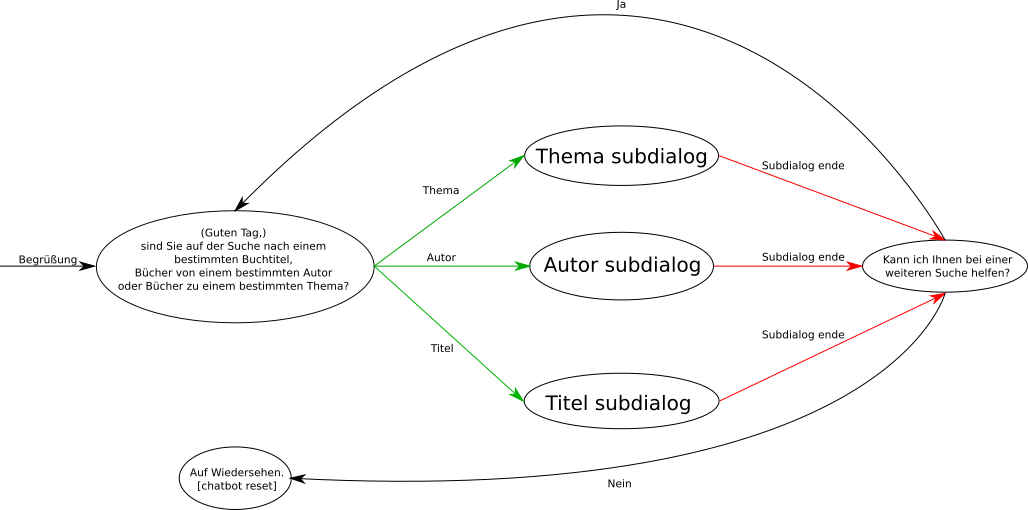
\includegraphics[width=\textwidth]{dialog_main.png}
    \caption{Übergreifende Dialogstruktur}
    \label{fig:main_dialog}
\end{figure}

\begin{figure}[ht]
    \centering
    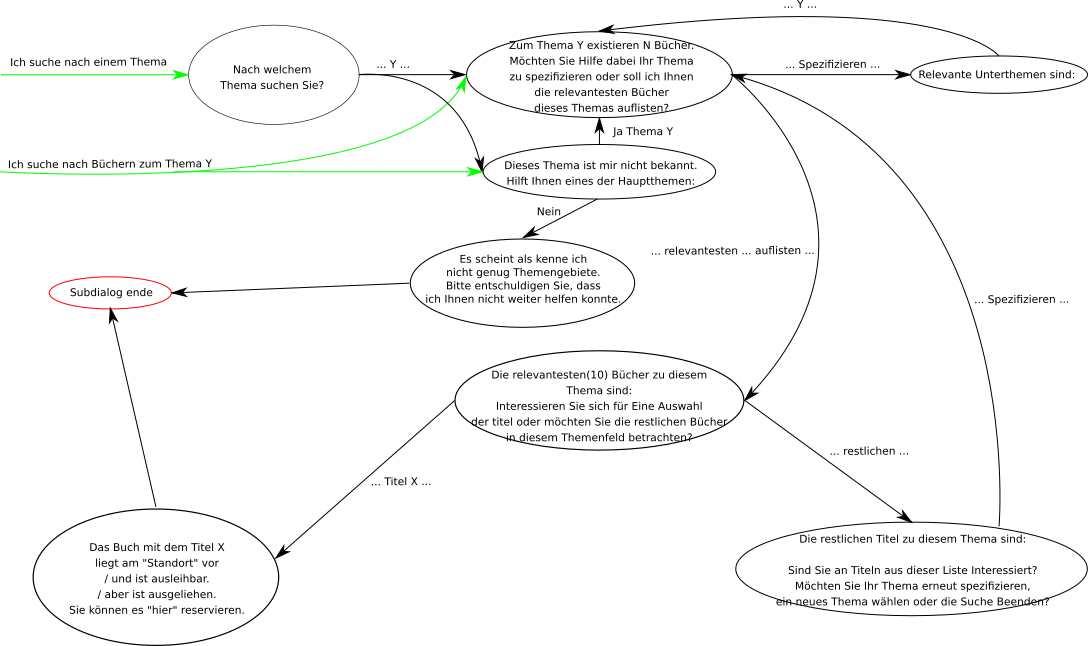
\includegraphics[width=\textwidth]{subdialog_theme.png}
    \caption{Themensuche Subdialog}
    \label{fig:category_subdialog}
\end{figure}

\begin{figure}[ht]
    \centering
    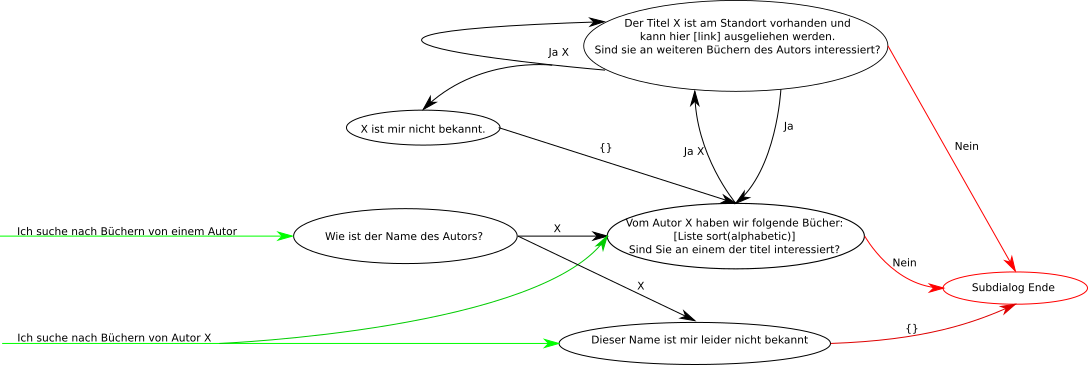
\includegraphics[width=\textwidth]{subdialog_author.png}
    \caption{Autorsuche Subdialog}
    \label{fig:author_subdialog}
\end{figure}

\begin{figure}[ht]
    \centering
    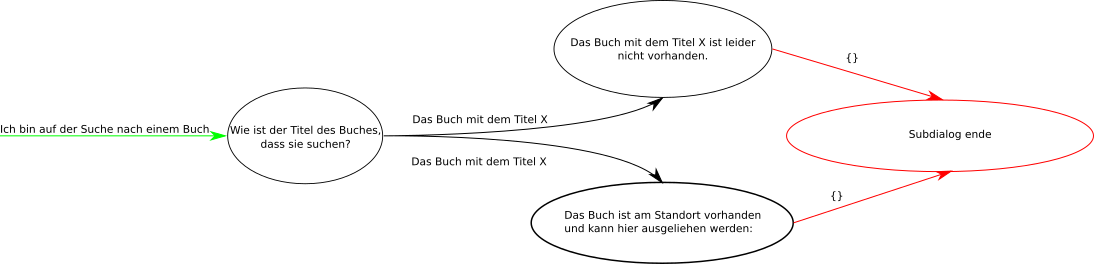
\includegraphics[width=\textwidth]{subdialog_title.png}
    \caption{Titelsuche Subdialog}
    \label{fig:title_subdialog}
\end{figure}

\begin{figure}[h]
    \centering
       \fbox{\begin{minipage}{13 cm}
            \begin{itemize}
                \item Bitte suchen Sie nach Büchern von Thomas Mann 
                \item Bitte suchen Sie nach Büchern über Magnetismus 
                \item Bitte suchen Sie nach dem Titel `' Eros und Mythos bei Plato ''
            \end{itemize}
        \end{minipage}} 
    \caption{Aufgaben für den Usability-Test}
    \label{fig:questions}
\end{figure}

\begin{figure}[ht]
    \centering
    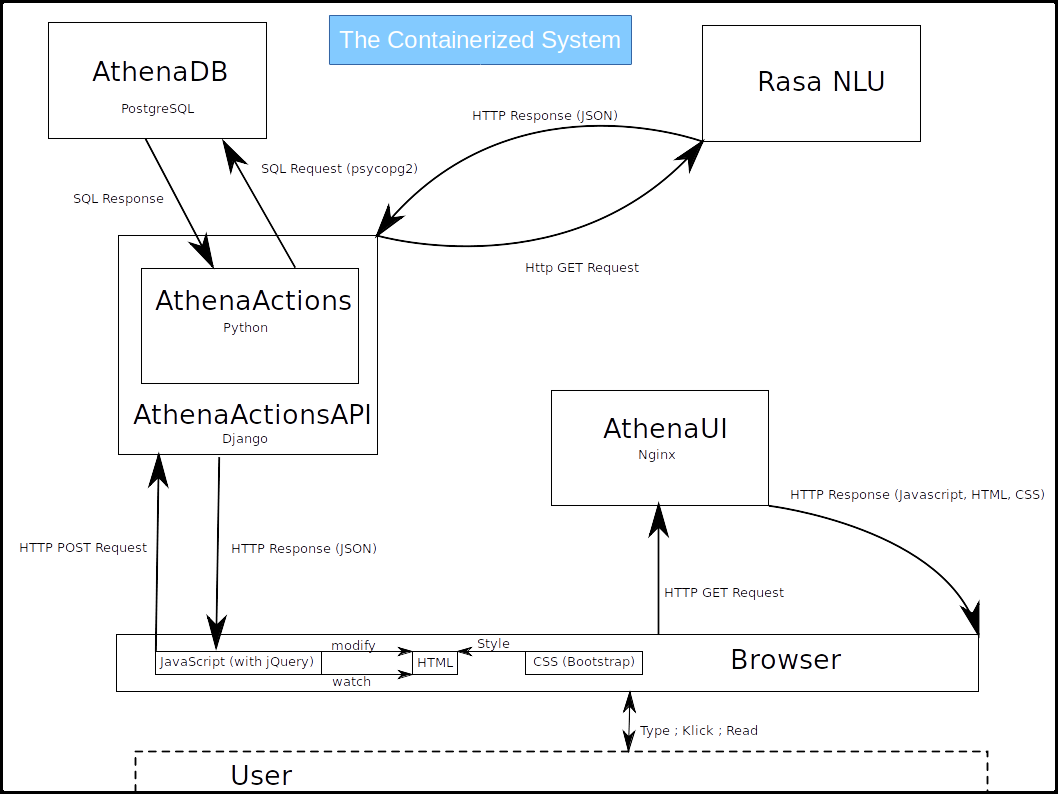
\includegraphics[width=\textwidth]{Athena_architecture.png}
    \caption{Athena Architektur}
    \label{fig:architecture_diagram}
\end{figure}

\begin{figure}[ht]
    \centering
    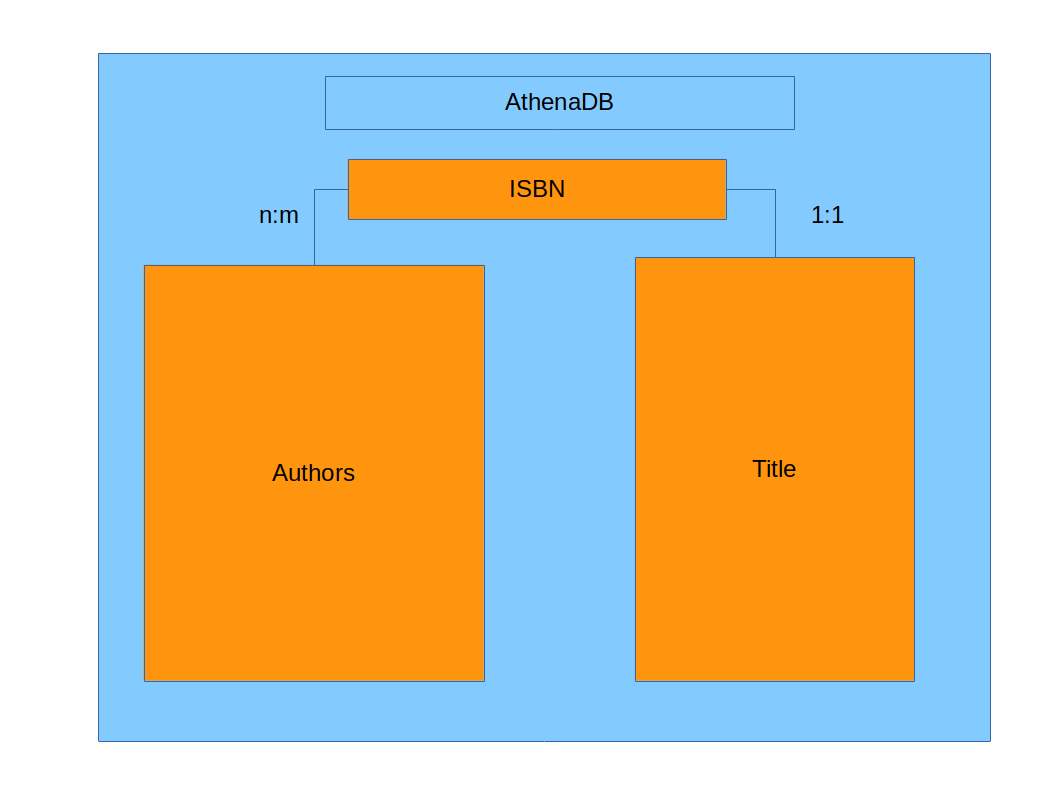
\includegraphics[width=\textwidth]{database_diag.png}
    \caption{Datenbank Tabellen}
    \label{fig:database_diagram}
\end{figure}

\begin{figure}[ht]
    \centering
    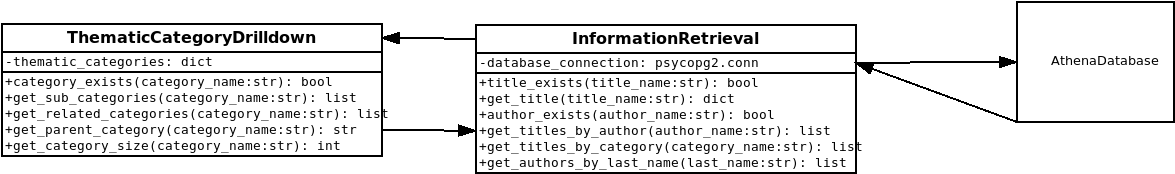
\includegraphics[width=\textwidth]{class_diag.png}
    \caption{AthenaActions Module mit Datenbank}
    \label{fig:class_diagram}
\end{figure}

\bibliography{bib}{}
\bibliographystyle{plain}

\end{document}
